\newpage

\section{机械结构设计}

\subsection{总体结构设计}

主要设计目标是设计一个自动车通用底盘:以“通用化”为核心特点,底盘被封装在一个扁平的车身中,未来将可以依据不同造型与功能需求,在云台位置搭载不同功能模块,如物流、快递、清扫、运输、甚至军警用特种装备等模块,成为适用于特定场景下各种功能的无人驾驶车辆。目前设计以搭载ZED双目摄像头,用于室内/外SLAM作为本设计的蓝本。

基本要求如下:长宽尺寸尺寸不超过 $ 1000mm \times 1000mm $的尺寸,实现简易有效的避震设计,传感器选用上采取模块化方法,并尽可能选取标准件,保障整体系统稳定性的实现。

首先将本机器人的命名确定为AtomIC(自动车通用底盘, \emph{Autonomous vehicle universal chassis})

因此我们由整体和功能的角度,结合抽象方法和模型方法的特征从总功能输入输出转换关系图,然后再建立分功能的结构简图,先画出最基本的功能即执行功能再画出他的输入和输出,最后图中各种流借助不同线型完成下方所示黑箱图。

\begin{figure}[htbp]
	\centering
	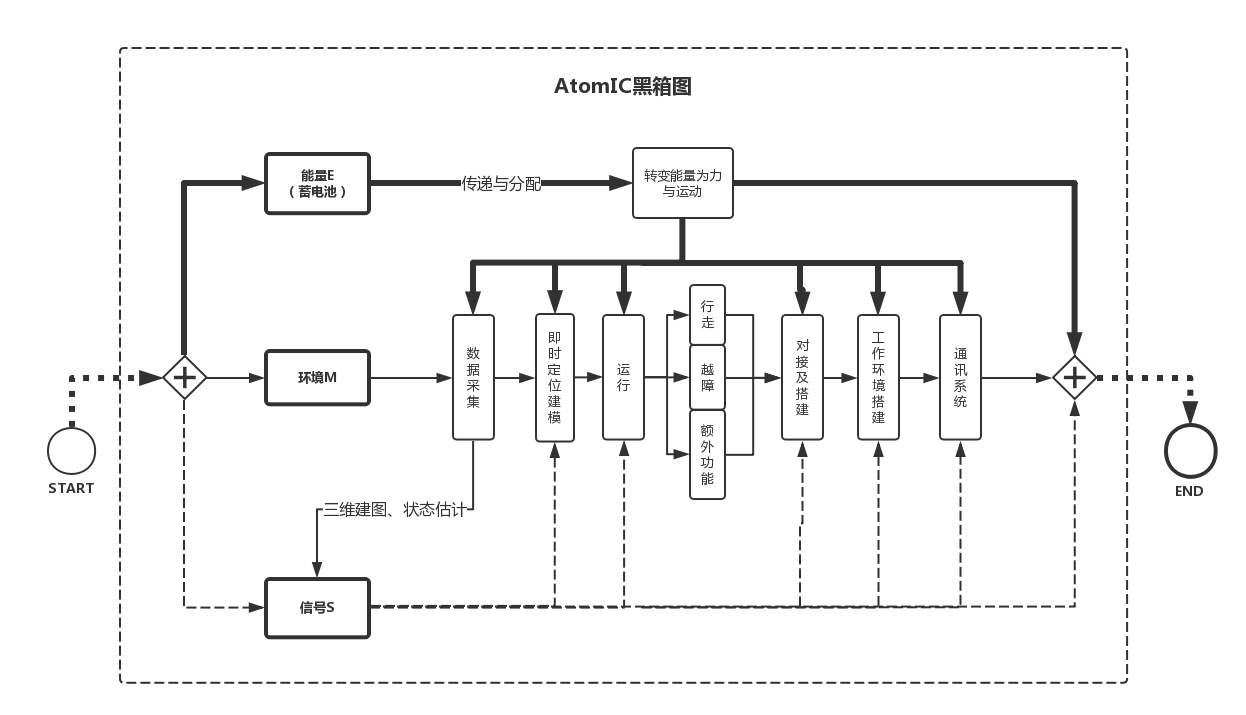
\includegraphics[width = 0.75\textwidth]{fig/hxt.png}
	\caption{功能黑箱图}
	\label{xtxjz}
\end{figure}

因此本无人车通用底盘的机械结构主要分为\textbf{车身主体,避震悬架,云台结构、电子元件保护结构以及其他结构}等结构,形态学矩阵如下图。

\begin{figure}[htbp]
	\centering
	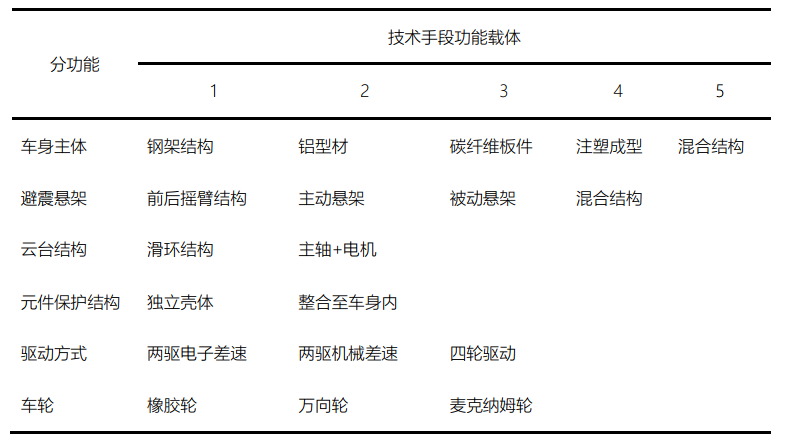
\includegraphics[width = 0.7\textwidth]{fig/xtxjz.png}
	\caption{形态学矩阵}
	\label{xtxjz}
\end{figure}

一共有多少$ 5 \times 4 \times 2 \times 2 \times 3 \times 3 =720 $种,而最终。在多种方案选择下,我们选取来这种"钢铝车身+碳纤维,被动避震,滑环结构、独立壳体、四轮驱动麦克纳姆轮"的方案。主要的优点如下:

\begin{enumerate}
	\item 对于车身主体方面,我们采用钢铝车身加工件与型材配合碳纤维主板的结构,这样的结构在保证强度的同时能够一定程度上保证轻量化与高效化;
	\item 被动避震、滑环结构的选择主要考虑是AtomIC平台主要应用于控制算法等相关云台模块的实现,在保证稳定耐用的前提下保证经济;
	\item 对于四轮驱动麦克纳姆轮的选择,这两者在目前已有很多成熟可靠的方案,并且四轮驱动和麦克纳姆轮在狭小空间与特定场景操作灵活并且具有可拓展性。
	
\end{enumerate}

以下就具体的机械结构进行说明与分析。

\subsection{细节模块选型设计}

\subsubsection{驱动轮选择}

麦克纳姆轮


\subsubsection{底盘机构设计}

底盘轮边避震结构


\subsubsection{云台机构设计}

to be continued


\subsection{机器人三维模型}

\begin{figure}[htbp]
	\centering
	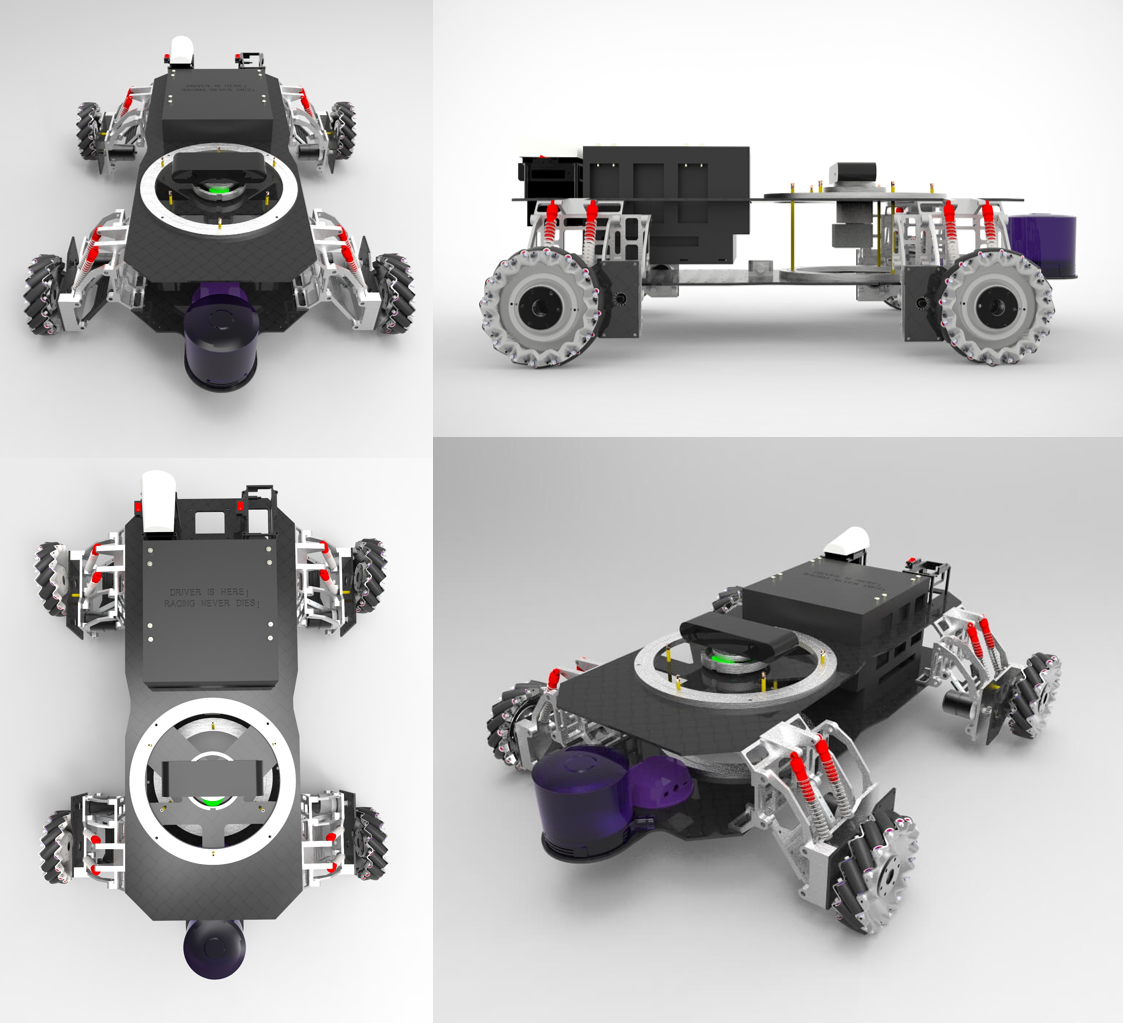
\includegraphics[width = 0.6\textwidth]{fig/xcsst.png}
	\caption{AtomIC渲染图}
	\label{xcsst}
\end{figure}

\begin{figure}[htbp]
	\centering
	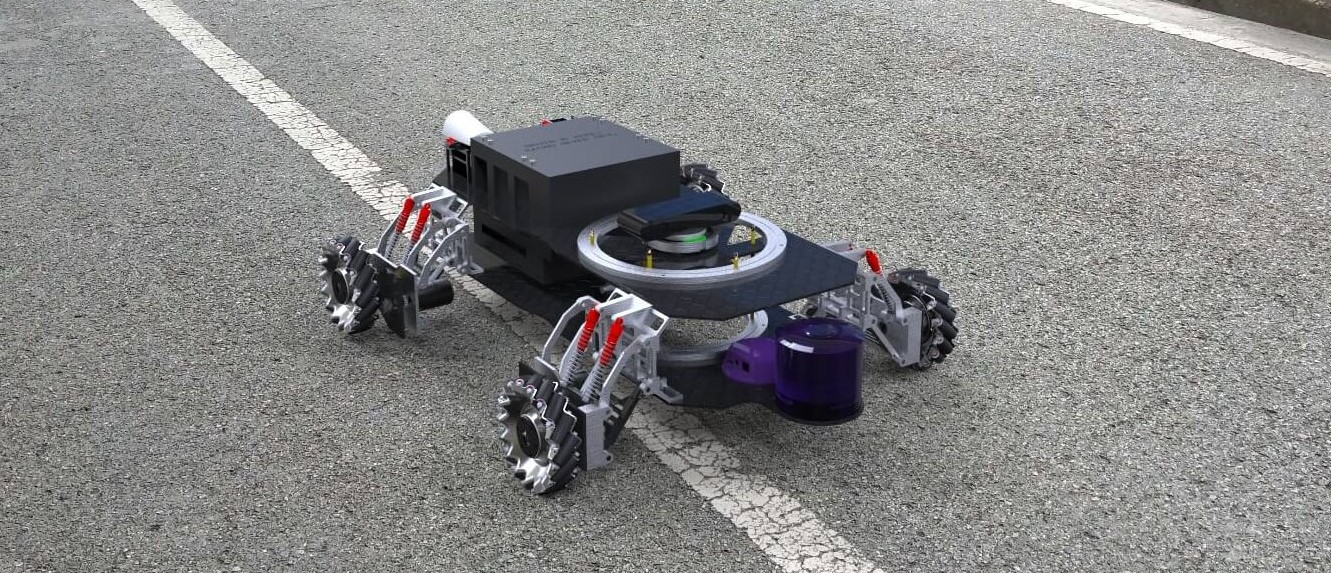
\includegraphics[width = 0.6\textwidth]{fig/jdgonglu.jpg}
	\caption{AtomIC公路场景渲染图}
	\label{jdgonglu}
\end{figure}


